% Chapter 1

\chapter{The basic safety hypervisor} % Main chapter title

\label{Chapter2} % For referencing the chapter elsewhere, use \ref{Chapter1} 

%----------------------------------------------------------------------------------------

% Define some commands to keep the formatting separated from the content 
%\newcommand{\keyword}[1]{\textbf{#1}}
%\newcommand{\tabhead}[1]{\textbf{#1}}
%\newcommand{\code}[1]{\texttt{#1}}
%\newcommand{\file}[1]{\texttt{\bfseries#1}}
%\newcommand{\option}[1]{\texttt{\itshape#1}}

%----------------------------------------------------------------------------------------

% IMPORTANT Add a section about IPC and interpartition communication
% IMPORTANT Do I talk enough about whether or not developers offer para or full or both?
% IMPORTANT Talk about supported hardware, v7 vs v8 and breadth of platforms

% IMPORTANT Maybe remove the intro fluff?
Now that the differences between traditional hypervisors and embedded safety hypervisors have been laid out, it is time to take a closer look at the embedded safety hypervisor.
For this, a "basic safety hypervisor" will be proposed, that embodies the typical characteristics of a microkernel based safety hypervisor. Where there is no discernible consensus, differences will be highlighted. Both the typical hypervisor architecture and its simplified functionality will be examined.

\section{Architecture}
Since, most safety hypervisors are microkernel based, the architecture for the basic safety hypervisor is also a more in-depth look at microkernel architecture. However, there are differences and additions to the microkernel core that will be explored as well.   

The guiding principle of microkernel design, minimality, has already been introduced in section\ref{microkernel}. But while the academic microkernel representations try to achieve \keyword{absolute minimality}, most real safety hypervisor implementations forego this to add useful features to the kernel. The small trusted code base is still an integral part of safety hypervisors, but with some minor trade-offs. 

% SOURCE Do I need a source for this?
Perhaps, the biggest trade-off is the inclusion of the virtual machine monitor code in the kernel itself. Some hypervisors also relegate this virtual machine control to user-space but it is more typical to see it inside of the microkernel. In reality the virtualization aspect of the hypervisor is almost always a critical component and it therefore makes sense to include it in the kernel verification efforts. 

\subsection{Capability-based access control}
% TODO Explain concept of least privilege
Capabilities are unforgeable tokens that grant access rights to an object. They contain the identification of the object and associated rights, for example read and write.
They can be given to other processes which in turn grants them access according to the capability \cite{Levy.1984}. A capability could be for a specific memory region, a communication endpoint or to a hypervisor \acrshort{api} call.

The capabilities a process has are maintained in a part of memory that it can not write, to stop the process from attempting to forge capabilities. It is however still up to the process to use the appropriate capability for access to reduce kernel involvement.

Capability-based access control has dominated in microkernels because of its flexibility and because it doesn't require extensive kernel involvement. Since, the typical safety hypervisor is an extension of a microkernel, this mechanism has propagated to them as well.

\subsection{Scheduling} \label{hv-scheduling}
All hypervisors implement some form of hierarchical scheduling, where a container task is scheduled that then schedules its children according to a global scheduling algorithm. This is most evident with virtualized operating systems. The hypervisor schedules the virtualized operating system according to the system configuration but how the \acrshort{os} in turn schedules its processes is up to the \acrshort{os}. Hierarchical scheduling can have the benefit of reducing scheduling slack in mixed criticality systems \cite{MalcolmS.Mollison.2010}. 

When it comes to how the container tasks are scheduled there is no single solution that is effective for every scenario. Consequently, the basic safety hypervisor offers different configurable scheduling behaviors. The two most common scheduling algorithms are preemptive priority based scheduling and time-sliced round-robin scheduling. Regardless of which algorithm is used, it needs to be deterministic to enable \acrlong{wcet} analysis. Without deterministic scheduling and \acrshort{wcet} analysis temporal separation can not be guaranteed and the system is unable to verifiably satisfy real-time requirements.

\paragraph{Preemptive priority based scheduling}
% FIGURE This might need one
In preemptive priority based scheduling each process has a priority and processes that are ready to be scheduled are scheduled based on their priority.
The preemptive means that if a process with a higher priority than the currently running process becomes ready to be executed, the currently running process gets interrupted. This ensures that the most critical task always gets the time it needs. If there are multiple processes with the same priority, the first to arrive gets scheduled first.

\paragraph{Time-sliced round-robin scheduling}
In time-sliced round-robin scheduling each process gets a dedicated time slice called a quantum. Figure \ref{fig:round_robin_example}  shows an example with three processes and their associated scheduling windows. If the end of the quantum is reached before the process is done, it gets interrupted and the next process is scheduled.
\begin{figure}
\centering
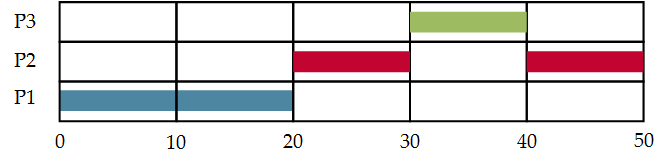
\includegraphics[scale=0.75]{Figures/round_robin_example.png}
\decoRule
\caption{An example for round robin scheduling}
\label{fig:round_robin_example}
\end{figure}

However, these were just the two most prevalent examples and in fact most hypervisors even allow the implementation of custom scheduling algorithms if the provided ones are not sufficient.

Another feature of the basic safety hypervisor is the possibility of multiple scheduling plans. A hypervisor partition with the correct capabilities is allowed to switch the scheduling behavior to one of the plans that was provided at configuration time. For example, if there is an unexpected error the monitoring partition can put the device into a maintenance mode, where only the most critical and recovery processes are scheduled. Another use for this feature is during the boot process where some partitions might need to run uninterrupted for a longer time.

\subsection{Available guest environments}
\subsubsection{\acrshort{rtos}}
Any safety hypervisor can host a \acrlong{rtos} as a guest environment, as it is one of the core objectives to separate real-time, safety-critical domains from the less critical domains. However, as explained in section \ref{hw-virt} (Hardware virtualization) the full virtualization of operating systems is not always available or feasible and in fact many hypervisors don't currently offer full virtualization. That leaves paravirtualization as the only option but paravirtualization requires the modification of the operating system in question. To reduce the barrier of entry the developer of the basic safety hypervisor typically also offers an already paravirtualized \acrshort{rtos} that can be deployed on the hypervisor. 

However, this significantly reduces the possible \acrshort{rtos} options the safety-critical device manufacturer can choose for his application. Since most real-time operating systems are closed source they cannot be modified to work on the hypervisor. This makes the \acrshort{rtos} provided by the hypervisor developer the potentially only viable option and therefore increases the dependence on the developer. What the potential consequences of this are needs to be evaluated based on the context of the situation but it is an important aspect to keep in mind.

\subsubsection{Linux}
An already paravirtualized version of Linux is another standard guest environment. Since, Linux is open-source the pressure of paravirtualization is not an immediate issue. Furthermore, there is less of a difference between versions of Linux than between real-time operating systems by different vendors. It is therefore unlikely that the safety-critical device manufacturer is even interested in using another version than the one provided.

\subsubsection{Native C runtime environment}
For a partition completing a very simple task, running a full-blown operating system is a waste of resources. For that reason the basic safety hypervisor includes a guest environment that is nothing more than a native C application with access to the hypervisor \acrshort{api}. The safety-critical device manufacturer can provide one or multiple C files that then get compiled into a hypervisor process. This process is then scheduled like any of the other partitions.

A possible application of this is a shared device driver. The driver can be implemented in the native C environment and communicate with the other partitions over the hypervisors \acrshort{ipc} mechanism. A more detailed explanation of this will be given in a future section.

%----------------------------------------------------------------------------------------

\section{Functionality}
This section will explore what functionality the safety hypervisor can offer and how it achieves this.
\subsection{Separation}
% IMPORTANT What about the other requirements of a sep-arch?!
The concepts of separation have been introduced in section \ref{separation-arch}. Now it will be detailed how the hypervisor in particular achieves this separation.
\subsubsection{Temporal separation}
How the hypervisor may schedule its partitions has already been explained in section \ref{hv-scheduling}. The most important property of a hypervisor scheduling algorithm that emerged from that was its determinism. If the algorithm is deterministic the device manufacturer can carry out a \acrshort{wcet} analysis, which allows him to reason about the device's temporal separation. The results of the \acrshort{wcet} analysis should show that even in the absolute worst case, the critical partitions still get the time they need to ensure the safety of the device. In all highly critical devices with real-time requirements this is a necessary step to achieve regulatory compliance.

Because the hypervisor has full control over the system it can stop or start processes at will. Through this, the hypervisor can make sure the schedule is kept and no process oversteps its boundaries.

% I kind of need to explain interrupts after I explain device access. And then I can also better explain how they are relevant to temporal separation
Another way for a partition to impact the timing behavior of another partition is through interrupts. Interrupts are the main way external peripherals communicate with the software on the device. They are 



* The ways of scheduling have already been detailed
* The hypervisor can achieve temporal separation because it has full control over the system and can force partitions to stop or start
* The deterministic scheduling behavior is also important to reason about the temporal separation
* Maybe go into more detail
* How are secondary timing problems solved (like interrupts etc.)
    -> I think I may be overcomplicating this issue
\subsubsection{Spatial separation}
% Same as with temporal
On most systems 

* DMA is only possible with IOMMU!

* It achieves this through utilizing the MMU or more rarely the MPU
* Some objects related to partitions need to be saved in kernel memory
* Either, partitions have a kernel memory quota or they can only instantiate objects that were defined at configuration time. This stops them from starving other processes of kernel memory
\subsection{Inter-partition communication}
There are two ways for two partitions to communicate: message passing and shared memory.

\subsubsection{Shared memory}
If two partitions are configured to share memory the hypervisor simply 

\subsubsection{Message passing}

* There are two ways to communicate with another partition: message passing and shared memory.
* In the shared memory case the hypervisor simply maps the same physical memory region into the virtual memory region of both partitions. The partitions then need to take care of everything else themselves. That means the partitions need to make sure they are not overwriting each others data and so on...
* Message passing is done through so called ports. Ports are defined at configuration time and have one source and one or more destinations. There are two types of ports: Queuing ports maintain a FIFO queue of messages that the consumer can take. In sampling ports a new message overwrites the existing one. 
* In the port scenario the hypervisor does have some control over the communication. [Explain what this means and what comes from it]
\subsubsection{User space synchronization}
* Some hypervisors may offer built-in synchronization mechanisms like semaphores to user space partitions
* This is especially useful if two partitions share memory and need to synchronize who is allowed to access it. 
\subsection{Partition privileges}
* At the very least there is two privilege levels. That of a system partition and a normal partition. A system partition is allowed to monitor and change the state of other partitions or the system as a whole. For example, it is allowed to execute the hypercall for shutting down another partition.
* There may also be more granular control where individual hypercalls can be allowed or disallowed
\subsection{Health monitoring}
* First events get detected. There are three types of events:
    -> Events caused by abnormal hardware behavior. The hypervisor is notified of this by processor traps
    -> Events detected and triggered by partition code. These are usually related to assertions or checks.
    -> Events triggered by the hypervisor itself. Usually because of a violation of a sanity check performed by the hypervisor. Either on the hypervisors internal state or that of a partition. This may also include a partition attempting to perform actions it is not allowed to
* A developer can then assign some basic actions that should follow a certain event, like restarting the partition or even the entire system. There doesn't have to be a defined action for everything.
* Simultaneously all events also get reported to the global log stream. Any partition with access to this stream can read it and may take more intricate steps to resolve the problem. This can be performed either as a replacement to the basic action described previously or on top of it.
* Add an image!
\subsection{Device access}
* To control a device, the partition needs control over the corresponding interrupt lines and device registers (typically handled by memory mapped IO on ARM and that or IO ports on x86)
* If only one partition needs access to a device it can be assigned directly.
* If devices are shared an IO Server partition needs to be implemented. It controls the device and gives access to the device over the inter-partition communication mechanism of the hypervisor. 
* Hardware interrupts can be assigned during configuration. 
* The hypervisor also often extends the interrupts there are with his own events. This can be used to notify partitions of hypervisor events like new messages at a queuing port for which they are a destination.
\subsection{Timers}
* Because the hypervisor can obfuscate a partitions view of time compared to if it was running on bare-metal (elaborate what this means), it offers virtual timers.
* The partition may either request the current time or activate a timer and receive an interrupt when the timer expires [...]
\subsection{Static configuration}
% NOTE Maybe this should be at the end of functionality section so I can give better examples for configuration
Configuration includes: 
* hardware resource access
* partition rights (ability to use restricted hypercalls)
* scheduling (with a caveat)
* partitions and what is running on them
* allowed communication paths

Any mechanism to modify a guest's rights at runtime, poses the risk of the system getting compromised, be it accidental or purposeful. For this reason dynamic configuration is not possible in the basic safety hypervisor. The only exception is the switching of scheduling plans by an authorized partition. But in this case all possible scheduling plans need to be defined at system design time and only these predefined scheduling plans can be activated.

That is why these systems are typically statically configured and if configuration runtime is at all possible, it is restricted to reducing privilege. For example, a guest that is allowed to spawn other guests may give them his own rights or less than his own but never more.
* Scheduling plans can usually be switched but only to predefined plans by authorized partitions. This

%----------------------------------------------------------------------------------------
\section{Initial considerations}
% TODO Rename this section
Although the considerations for choosing a hypervisor implementation will be outlined later in the thesis, in section \ref{how-to-decide}, some crucial factors need to be elaborated here to avoid confusion.
\subsection{First- or third-party hypervisor}
A manufacturer has the option to either license a third-party hypervisor or develop his own solution. The development costs of a third-party hypervisor are effectively shared with many parties over the course of many projects, whereas the development costs of a first-party hypervisor are typically only shared over the course of many projects in a single company. However, developing one's own hypervisor provides the maximum amount of control over functionality and development cycle.

Additionally, it means that the best possible subject matter experts on the hypervisor are always available to the manufacturer. But here also lies another big problem: Developing a custom hypervisor not only requires the initial development costs but also the costs of hiring or developing the talent required. A third-party already has these capacities and can therefore also typically go beyond the absolute necessity in terms of functionality.

Ultimately, the more prudent approach is probably licensing a third-party hypervisor but in some cases it may be beneficial to have full control over the environment. 

\subsection{Security}
Security will not be a consideration in this thesis, only a word of warning will be issued. It may seem logical to assume that a hypervisor can provide security as well as safety and while it may not initially be a bad idea to have separation between security-critical and non-security-critical software it is not that simple. A hypervisor offers a much greater attack incentive, as a compromisation of the platform could be used to attack a lot of different devices. It is also questionable whether or not the goals of security and safety align. A manufacturer doesn't want to modify a certified device or at least do it in bulk to minimize the cost of recertification. Building a secure device on the other hand often requires frequent updates to fix newly found attack vectors. So the security of any given hypervisor implementation should not be taken for granted and analyzed with scrutiny.
%----------------------------------------------------------------------------------------

\section{Limitations}
Before getting into the full-fledged analysis it is best to expose some limitations of the current safety hypervisor landscape. 
\subsection{Current hardware restrictions}
Hypervisors are overall still limited to the more powerful \keyword{application processors} and have not really penetrated the \keyword{microcontroller} market. Using a hypervisor is also not possible if a specialized processor, like a \acrfull{dsp}, will be the only processor in the system. Although, this restriction may be lifted in the future.  There are several reasons for the hypervisor's hardware restrictions. 

% PHRASING 
First of all, microcontrollers typically have no \acrshort{mmu} only an \acrshort{mpu} or no memory protection at all. Hypervisors need at least some hardware memory protection, as the corresponding software isolation is far too slow. \acrshort{mpu}s have a limited number of partitions they can isolate and therefore impose uncomfortable restrictions on hypervisor developers and users.

Second, the hardware virtualization extensions are not yet available on microcontrollers. And even though the typical safety hypervisor prefers paravirtualized guests, virtualization extensions are still beneficial for preventing the guest from doing things it is not supposed to. ARM, for example, offers a trap mechanism that allows the hypervisor to disable certain instructions and special registers for the guest \cite{ARM.v8.2018}. 

And finally, a hypervisor is fundamentally about isolating software components from each other. It is more likely that this is necessary on a stronger processor and not on a microcontroller.

However, with all of these restrictions laid out, there are developments that aim to make hypervisors viable on microcontrollers. Read more about this in section \ref{tech-progress}.

\subsection{Effective multicore isolation}
% NOTE Maybe add a graphic
Imagine a system with two partitions, one safety-critical one not safety-critical, that runs on a two-core \acrshort{cpu} with a shared cache between the two cores. During its allocated time the safety-critical partition may fill up the cache with relevant values. Once the non-safety-critical software runs it can evict all of the cache values by populating it with its own values. This can lead to large and potentially unpredictable interference across domains \cite{AlessandroBiondi.2018}.

In the best case this scenario just leads to an excessively pessimistic \acrfull{wcet} analysis and to compensate this the safety-critical partition would get a lot more allocated time than it actually needed, leading to a worse average case performance. There are efforts to solve this issue reliably \cite{PaoloModica.2018}.

%----------------------------------------------------------------------------------------

